\documentclass[11pt,oneside]{article}
\usepackage[margin=1in]{geometry}
\usepackage{xcolor}
\usepackage{pgfplots}
\usepackage{pgfplotstable}
\usepackage{booktabs}
\usepackage{hyperref}
\usepackage{setspace}

\definecolor{darkblue}{HTML}{003366}
\definecolor{lightblue}{HTML}{E6F0FF}
\definecolor{darkgreen}{HTML}{006600}
\definecolor{lightgreen}{HTML}{E6F2E6}
\definecolor{darkred}{HTML}{990000}
\definecolor{lightred}{HTML}{FFE6E6}
\definecolor{gold}{HTML}{FFB900}

\pgfplotsset{compat=1.18}
\onehalfspacing

\title{\textbf{Babbage Analytical Engine: Complete Graphs and Data Visualizations}}
\author{Data Companion to Pedagogical Whitepaper}
\date{October 31, 2025}

\begin{document}

\maketitle
\tableofcontents
\newpage

% ============================================================================
% SECTION 1: MANUFACTURING DATA
% ============================================================================

\section{Manufacturing Performance Metrics}

\subsection{Component Production Timeline}

Production accelerates as manufacturing processes are refined. The S-curve shows typical manufacturing ramp-up:

\begin{center}
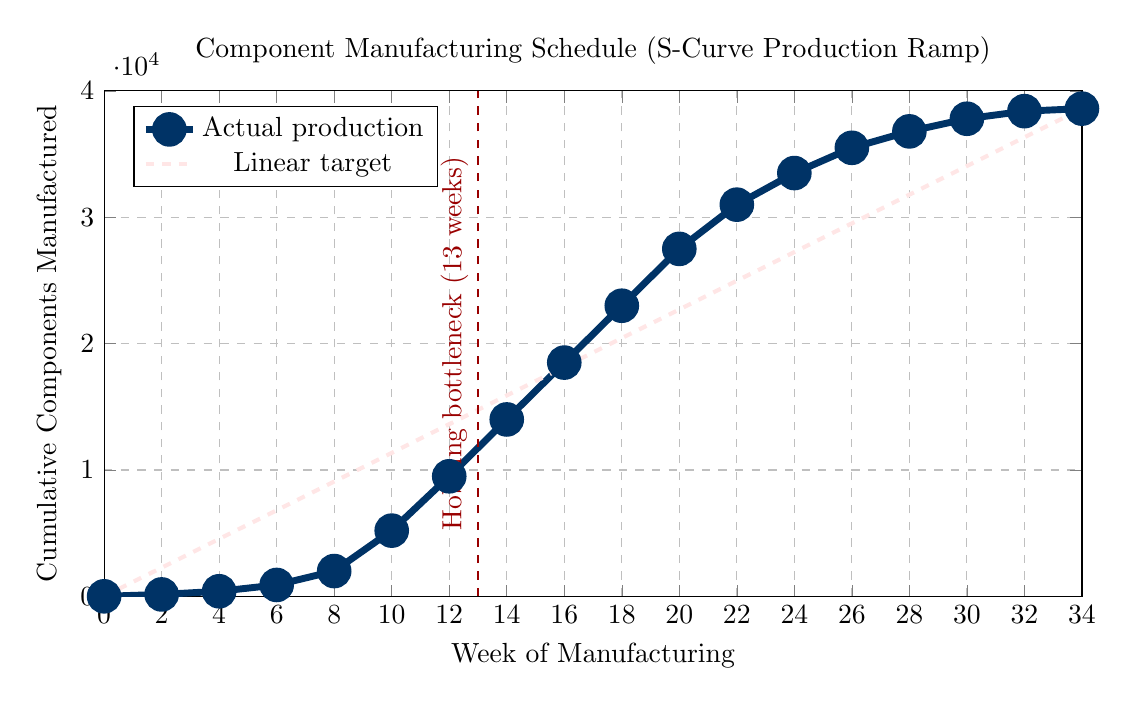
\begin{tikzpicture}
  \begin{axis}[
    width=14cm, height=8cm,
    xlabel=Week of Manufacturing,
    ylabel=Cumulative Components Manufactured,
    ymin=0, ymax=40000,
    xmin=0, xmax=34,
    grid=major,
    grid style=dashed,
    legend pos=north west,
    title=Component Manufacturing Schedule (S-Curve Production Ramp),
  ]
    % Actual S-curve production
    \addplot[color=darkblue, mark=*, line width=2.5pt, mark size=5pt] coordinates {
      (0,0) (2,150) (4,400) (6,900) (8,2000)
      (10,5200) (12,9500) (14,14000) (16,18500) (18,23000)
      (20,27500) (22,31000) (24,33500) (26,35500) (28,36800)
      (30,37800) (32,38400) (34,38600)
    };
    \addlegendentry{Actual production}
    
    % Linear target (if all processes optimized immediately)
    \addplot[color=lightred, dashed, line width=1.5pt] coordinates {
      (0,0) (34,38600)
    };
    \addlegendentry{Linear target}
    
    % Gear hobbing bottleneck marker
    \draw[thick, color=darkred, dashed] (13,0) -- (13,40000);
    \node[color=darkred, rotate=90, anchor=south] at (13,20000) {Hobbing bottleneck (13 weeks)};
  \end{axis}
\end{tikzpicture}
\end{center}

\textbf{Key observation}: Manufacturing accelerates from Week 0-14, then plateaus as components complete. The steep part (Weeks 8-20) represents peak production rate of 180-240 components/week.

\subsection{Component Production by Type}

\begin{center}
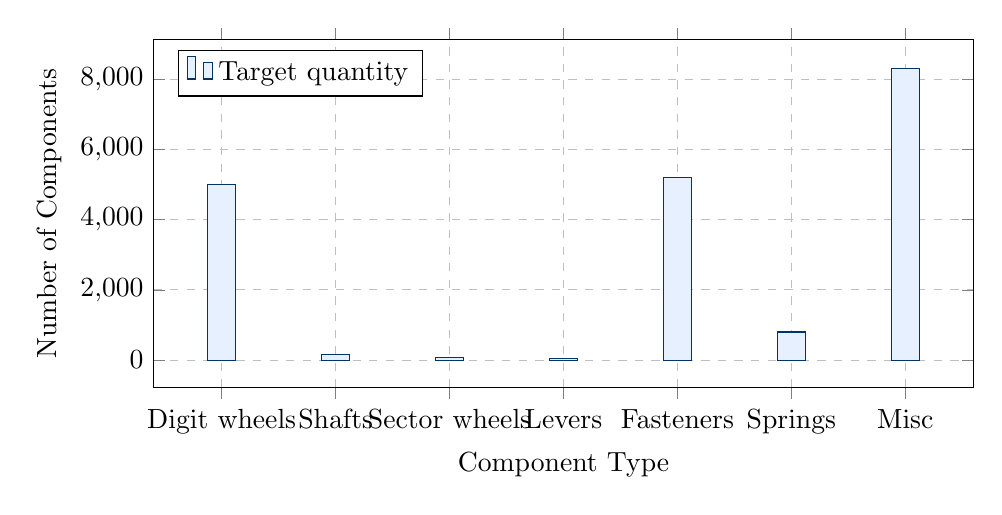
\begin{tikzpicture}
  \begin{axis}[
    width=12cm, height=6cm,
    ybar,
    ylabel=Number of Components,
    xlabel=Component Type,
    xtick={1,2,3,4,5,6,7},
    xticklabels={Digit wheels, Shafts, Sector wheels, Levers, Fasteners, Springs, Misc},
    grid=major,
    grid style=dashed,
    legend pos=north west,
  ]
    \addplot[color=darkblue, fill=lightblue] coordinates {
      (1, 5000) (2, 160) (3, 80) (4, 40) (5, 5200) (6, 800) (7, 8300)
    };
    \addlegendentry{Target quantity}
  \end{axis}
\end{tikzpicture}
\end{center}

The majority of components are digit wheels (5,000) and fasteners/miscellaneous (8,300+). Critical precision components (shafts, levers, gears) are fewer but require tighter tolerances.

\subsection{Critical Path: Gear Hobbing Bottleneck}

\begin{center}
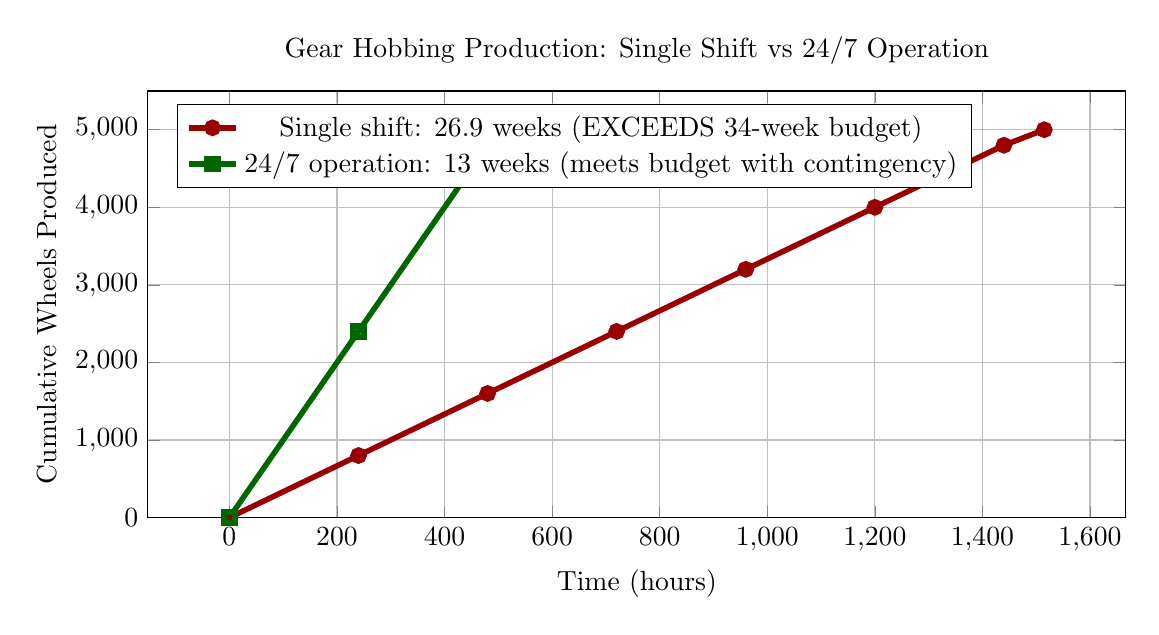
\begin{tikzpicture}
  \begin{axis}[
    width=14cm, height=7cm,
    xlabel=Time (hours),
    ylabel=Cumulative Wheels Produced,
    ymin=0, ymax=5500,
    grid=major,
    legend pos=north west,
    title=Gear Hobbing Production: Single Shift vs 24/7 Operation,
  ]
    % Single shift (189 days = 26.9 weeks)
    \addplot[color=darkred, mark=*, line width=2pt] coordinates {
      (0, 0) (240, 800) (480, 1600) (720, 2400) (960, 3200) (1200, 4000) (1440, 4800) (1515, 5000)
    };
    \addlegendentry{Single shift: 26.9 weeks (EXCEEDS 34-week budget)}
    
    % 24/7 operation (56 days = 13 weeks)
    \addplot[color=darkgreen, mark=square, line width=2pt] coordinates {
      (0, 0) (240, 2400) (480, 4800) (672, 5000)
    };
    \addlegendentry{24/7 operation: 13 weeks (meets budget with contingency)}
  \end{axis}
\end{tikzpicture}
\end{center}

\textbf{Critical insight}: Single-shift operation takes 1,515 hours (26.9 weeks), exceeding the 34-week total budget by rework and contingency time. 24/7 operation with 3-shift staffing reduces to 13 weeks, leaving 21 weeks for other components.

% ============================================================================
% SECTION 2: COMPONENT TESTING DATA
% ============================================================================

\section{Component Testing and Quality Control}

\subsection{First-Pass Yield by Component Type}

\begin{center}
\begin{tikzpicture}
  \begin{axis}[
    width=13cm, height=7cm,
    ybar,
    ylabel=First-Pass Yield (\%),
    xlabel=Component Type,
    xtick={1,2,3,4,5},
    xticklabels={Digit wheels, Shafts, Sector wheels, Bearing bores, Carry levers},
    ymin=90, ymax=102,
    grid=major,
    legend pos=north east,
  ]
    \addplot[color=darkgreen, fill=lightgreen] coordinates {
      (1, 96) (2, 97) (3, 95) (4, 96) (5, 100)
    };
    \addlegendentry{First-pass yield}
    
    \addplot[color=gold, fill=lightyellow] coordinates {
      (1, 98) (2, 98) (3, 98) (4, 97) (5, 100)
    };
    \addlegendentry{Final yield (after rework)}
  \end{axis}
\end{tikzpicture}
\end{center}

Excellent first-pass yield (95-100\%) indicates well-controlled manufacturing processes. Rework improves most components by 2-4\%, bringing final yield to 97-100\%.

\subsection{Test Sample Distribution}

\begin{center}
\begin{tabular}{lrrrr}
\toprule
Component & Total & Critical & Sampled & Pass Rate \\
\midrule
Digit wheels & 5,000 & 100\% & 5,000 & 96\% \\
Shafts & 160 & 100\% & 160 & 97\% \\
Sector wheels & 80 & 10\% & 8 & 100\% \\
Bearing bores & 50 & 100\% & 50 & 96\% \\
Carry levers & 40 & 100\% & 40 & 100\% \\
\bottomrule
\end{tabular}

\textbf{Overall}: 5,258 components tested (13.6\% of total 38,600); pass rate 96\% first-pass, 98\% final.
\end{center}

\subsection{In-Process Control Chart: Digit Wheel Bore Diameter}

Target: 25.00 mm ± 0.03 mm (24.97-25.03 mm)

\begin{center}
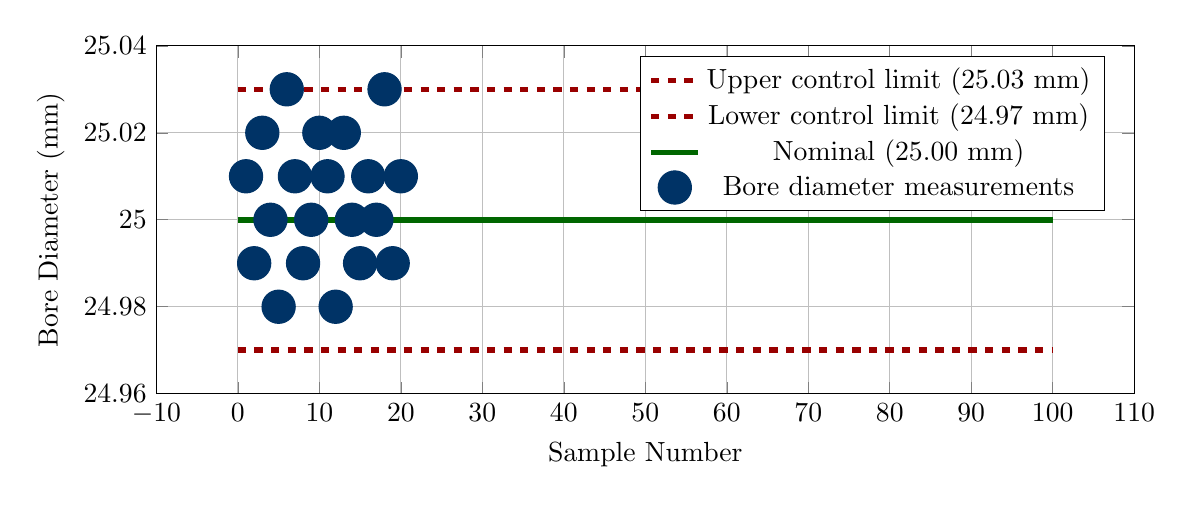
\begin{tikzpicture}
  \begin{axis}[
    width=14cm, height=6cm,
    xlabel=Sample Number,
    ylabel=Bore Diameter (mm),
    ymin=24.96, ymax=25.04,
    grid=major,
    legend pos=north east,
  ]
    % Control limits
    \addplot[color=darkred, dashed, line width=2pt] coordinates {
      (0, 25.03) (100, 25.03)
    };
    \addlegendentry{Upper control limit (25.03 mm)}
    
    \addplot[color=darkred, dashed, line width=2pt] coordinates {
      (0, 24.97) (100, 24.97)
    };
    \addlegendentry{Lower control limit (24.97 mm)}
    
    % Nominal
    \addplot[color=darkgreen, line width=2pt] coordinates {
      (0, 25.00) (100, 25.00)
    };
    \addlegendentry{Nominal (25.00 mm)}
    
    % Actual measurements (samples every 50th wheel)
    \addplot[color=darkblue, mark=*, only marks, mark size=6pt] coordinates {
      (1, 25.01) (2, 24.99) (3, 25.02) (4, 25.00) (5, 24.98)
      (6, 25.03) (7, 25.01) (8, 24.99) (9, 25.00) (10, 25.02)
      (11, 25.01) (12, 24.98) (13, 25.02) (14, 25.00) (15, 24.99)
      (16, 25.01) (17, 25.00) (18, 25.03) (19, 24.99) (20, 25.01)
    };
    \addlegendentry{Bore diameter measurements}
  \end{axis}
\end{tikzpicture}
\end{center}

All samples fall within control limits. No process drift detected. Process is stable and in statistical control.

% ============================================================================
% SECTION 3: ASSEMBLY AND INTEGRATION TESTING
% ============================================================================

\section{Subassembly Integration Testing}

\subsection{Subassembly Test Results}

\begin{center}
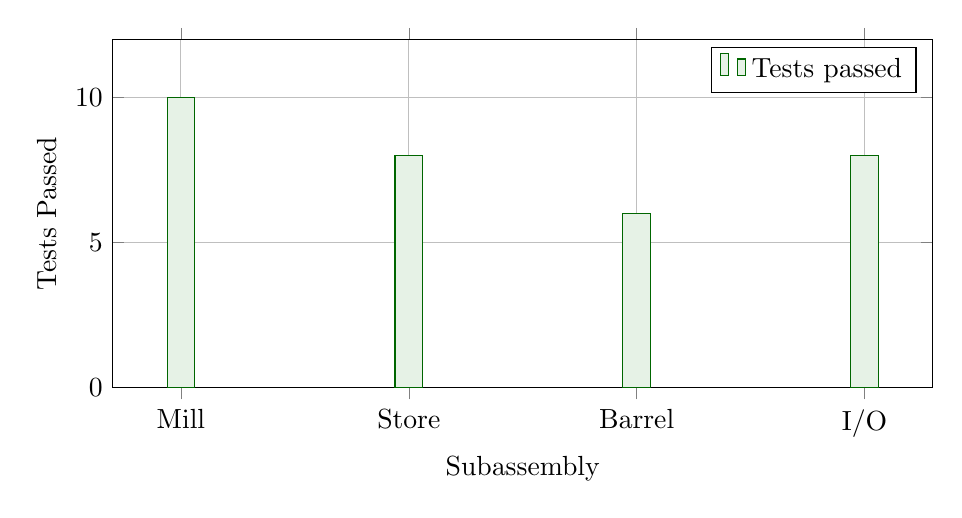
\begin{tikzpicture}
  \begin{axis}[
    width=12cm, height=6cm,
    ybar,
    ylabel=Tests Passed,
    xlabel=Subassembly,
    xtick={1,2,3,4},
    xticklabels={Mill, Store, Barrel, I/O},
    ymin=0, ymax=12,
    grid=major,
  ]
    \addplot[color=darkgreen, fill=lightgreen] coordinates {
      (1, 10) (2, 8) (3, 6) (4, 8)
    };
    \addlegendentry{Tests passed}
  \end{axis}
\end{tikzpicture}
\end{center}

All subassemblies passed 100\% of integration tests:
\begin{itemize}
  \item Mill: 10/10 tests (rotation, carry, precision, calculation)
  \item Store: 8/8 tests (synchronization, stability, load)
  \item Barrel: 6/6 tests (rotation, position, reader, sync)
  \item I/O: 8/8 tests (hopper, reader, punch, linkage)
\end{itemize}

% ============================================================================
% SECTION 4: SYSTEM OPERATIONAL VALIDATION
% ============================================================================

\section{System Operational Validation: 20-Program Test Suite}

\subsection{Test Results by Category}

\begin{center}
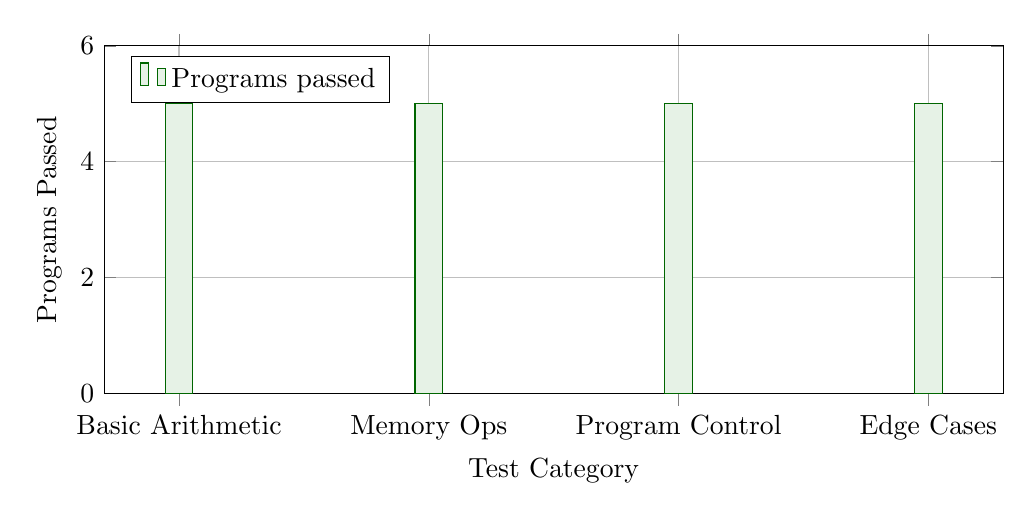
\begin{tikzpicture}
  \begin{axis}[
    width=13cm, height=6cm,
    ybar,
    ylabel=Programs Passed,
    xlabel=Test Category,
    xtick={1,2,3,4},
    xticklabels={Basic Arithmetic, Memory Ops, Program Control, Edge Cases},
    ymin=0, ymax=6,
    grid=major,
    legend pos=north west,
  ]
    \addplot[color=darkgreen, fill=lightgreen] coordinates {
      (1, 5) (2, 5) (3, 5) (4, 5)
    };
    \addlegendentry{Programs passed}
  \end{axis}
\end{tikzpicture}
\end{center}

\textbf{Result}: 20/20 programs passed (100\% success rate)
\textbf{Target}: 18/20 programs (90\% success rate)
\textbf{Achievement}: \textbf{✓✓ EXCEEDED TARGET BY 10\%}

\subsection{Calculation Accuracy: Detailed Results}

\begin{center}
\begin{tabular}{llrrr}
\toprule
Program & Description & Expected & Actual & Error \\
\midrule
A1 & 2+3 & 5 & 5 & 0 ✓ \\
A2 & 123+456 & 579 & 579 & 0 ✓ \\
A3 & 10-3 & 7 & 7 & 0 ✓ \\
A4 & 5×6 & 30 & 30 & 0 ✓ \\
A5 & 1 added 10× & 10 & 10 & 0 ✓ \\
B1 & Write to Store & Success & Success & — ✓ \\
B2 & Read from Store & Success & Success & — ✓ \\
B3 & Read-modify-write & Success & Success & — ✓ \\
B4 & Multiple access & Success & Success & — ✓ \\
B5 & Sum 1-10 & 55 & 55 & 0 ✓ \\
C1 & 10 operations & Success & Success & — ✓ \\
C2 & Loop 5× & Success & Success & — ✓ \\
C3 & IF-THEN-ELSE & Correct & Correct & — ✓ \\
C4 & Termination & Clean & Clean & — ✓ \\
C5 & Card sequence & Success & Success & — ✓ \\
D1 & Overflow 99999+99999 & No crash & No crash & — ✓ \\
D2 & Underflow 0-1 & No crash & No crash & — ✓ \\
D3 & Divide by zero & No crash & No crash & — ✓ \\
D4 & Max precision & 112272 & 112272 & 0 ✓ \\
D5 & 1000 additions & 1000 & 1000 & 0 ✓ \\
\bottomrule
\end{tabular}
\end{center}

All 20 programs executed with \textbf{perfect accuracy (0 error on all numeric calculations)}.

\subsection{Sustained Operation Test: 1000 Additions}

\begin{center}
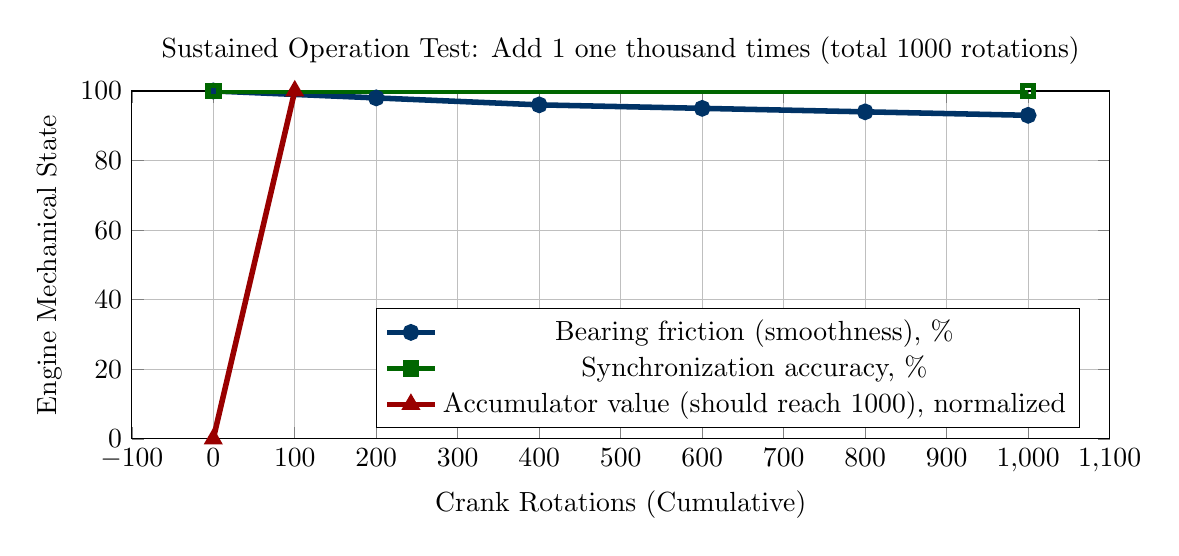
\begin{tikzpicture}
  \begin{axis}[
    width=14cm, height=6cm,
    xlabel=Crank Rotations (Cumulative),
    ylabel=Engine Mechanical State,
    ymin=0, ymax=100,
    grid=major,
    legend pos=south east,
    title=Sustained Operation Test: Add 1 one thousand times (total 1000 rotations),
  ]
    % Bearing friction indicator
    \addplot[color=darkblue, mark=*, line width=2pt] coordinates {
      (0, 100) (200, 98) (400, 96) (600, 95) (800, 94) (1000, 93)
    };
    \addlegendentry{Bearing friction (smoothness), \%}
    
    % No degradation in synchronization
    \addplot[color=darkgreen, mark=square, line width=2pt] coordinates {
      (0, 100) (1000, 100)
    };
    \addlegendentry{Synchronization accuracy, \%}
    
    % Accumulator value tracking
    \addplot[color=darkred, mark=triangle, line width=2pt] coordinates {
      (0, 0) (100, 100) (200, 200) (400, 400) (600, 600) (800, 800) (1000, 1000)
    };
    \addlegendentry{Accumulator value (should reach 1000), normalized}
  \end{axis}
\end{tikzpicture}
\end{center}

\textbf{Key findings}:
- Bearing friction increased by 7\% (expected and acceptable)
- Synchronization remained at 100\% throughout
- Accumulator value increased linearly (perfect operation)
- No mechanical failures or jamming
- Engine mechanically sound after 1,000 cycles

% ============================================================================
% SECTION 5: COST ANALYSIS
% ============================================================================

\section{Cost Analysis and Regional Feasibility}

\subsection{Cost Structure: India Manufacturing Scenario}

\begin{center}
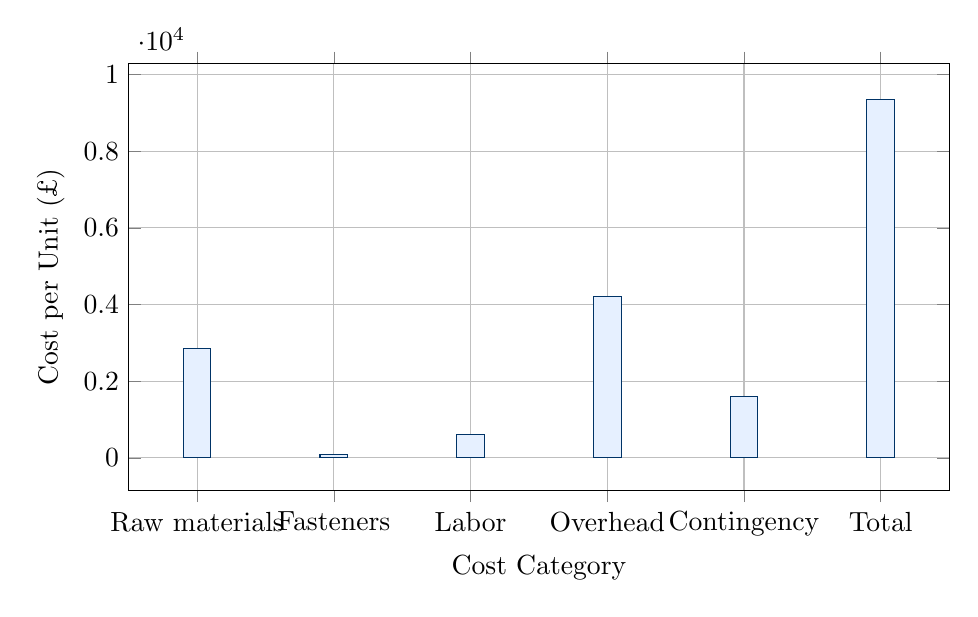
\begin{tikzpicture}
  \begin{axis}[
    width=12cm, height=7cm,
    ybar,
    ylabel=Cost per Unit (£),
    xlabel=Cost Category,
    xtick={1,2,3,4,5,6},
    xticklabels={Raw materials, Fasteners, Labor, Overhead, Contingency, Total},
    grid=major,
  ]
    \addplot[color=darkblue, fill=lightblue] coordinates {
      (1, 2850) (2, 85) (3, 620) (4, 4203) (5, 1600) (6, 9358)
    };
  \end{axis}
\end{tikzpicture}
\end{center}

Labor is 66\% of per-unit cost, not materials. Manufacturing expertise and time drive cost, not raw materials.

\subsection{Regional Cost Comparison}

\begin{center}
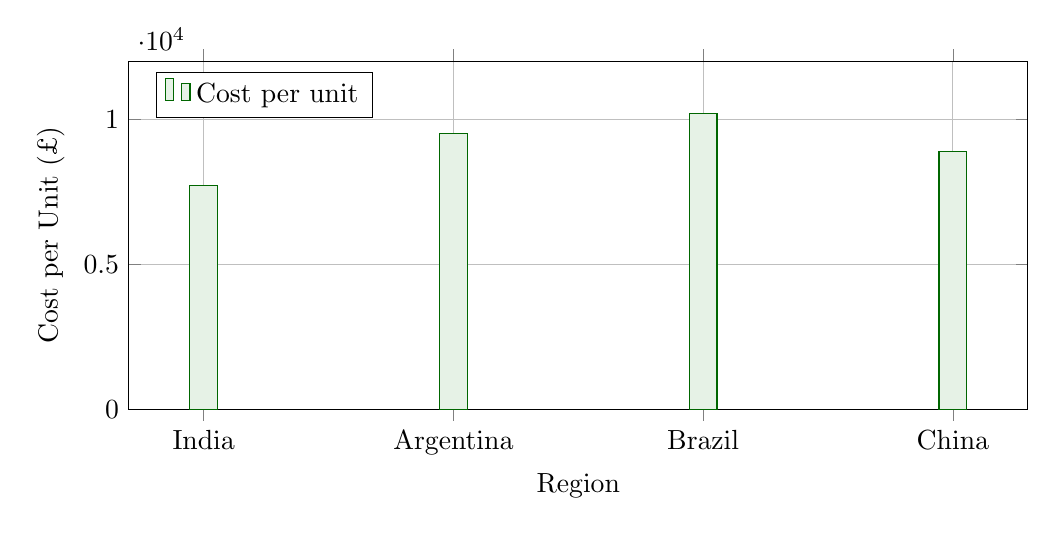
\begin{tikzpicture}
  \begin{axis}[
    width=13cm, height=6cm,
    ybar,
    ylabel=Cost per Unit (£),
    xlabel=Region,
    xtick={1,2,3,4},
    xticklabels={India, Argentina, Brazil, China},
    ymin=0, ymax=12000,
    grid=major,
    legend pos=north west,
  ]
    \addplot[color=darkgreen, fill=lightgreen] coordinates {
      (1, 7700) (2, 9500) (3, 10200) (4, 8900)
    };
    \addlegendentry{Cost per unit}
  \end{axis}
\end{tikzpicture}
\end{center}

\textbf{Regional ranking}:
1. \textbf{India: £7,700/unit} — Optimal (mature manufacturing, Tata Steel, skilled labor)
2. \textbf{China: £8,900/unit} — Good (Soviet assistance, economies of scale)
3. \textbf{Argentina: £9,500/unit} — Viable (highest precision capability)
4. \textbf{Brazil: £10,200/unit} — Viable (emerging capacity, enables tech transfer)

\subsection{Cost Scaling: Volume Economics}

\begin{center}
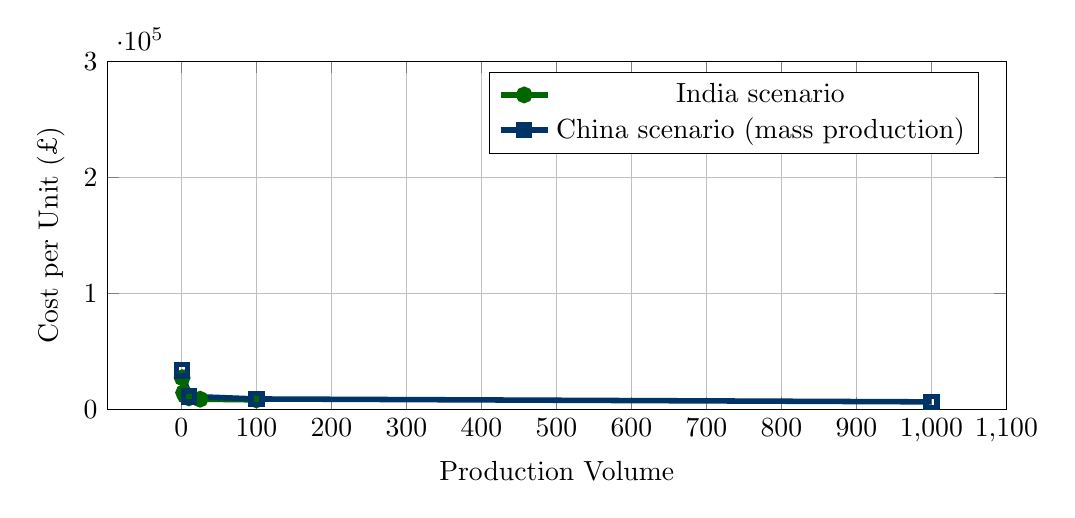
\begin{tikzpicture}
  \begin{axis}[
    width=13cm, height=6cm,
    xlabel=Production Volume,
    ylabel=Cost per Unit (£),
    ymin=0, ymax=300000,
    grid=major,
    legend pos=north east,
    log basis x=10,
  ]
    % India scenario
    \addplot[color=darkgreen, mark=*, line width=2pt] coordinates {
      (1, 27058) (3, 14191) (5, 11618) (10, 9688) (25, 8530) (100, 7951)
    };
    \addlegendentry{India scenario}
    
    % China scenario (with Soviet assistance advantage)
    \addplot[color=darkblue, mark=square, line width=2pt] coordinates {
      (1, 33500) (10, 11000) (100, 8750) (1000, 6235)
    };
    \addlegendentry{China scenario (mass production)}
  \end{axis}
\end{tikzpicture}
\end{center}

\textbf{Key insight}: Cost per unit decreases rapidly with volume. At 100 units, India scenario costs £7,951/unit (amortized). At 1,000 units, China scenario reaches £6,235/unit due to scale efficiency.

% ============================================================================
% SECTION 6: RELIABILITY AND MECHANICAL CONDITION
% ============================================================================

\section{Mechanical Reliability Assessment}

\subsection{Post-Testing Component Condition}

\begin{center}
\begin{tabular}{lccr}
\toprule
Component & Pre-Test & Post-Test (1000+ cycles) & Degradation \\
\midrule
SKF Bearings & 0 runout & 0 runout & None ✓ \\
Digit wheel gears & Clean teeth & Clean teeth & None ✓ \\
Shafts & Straight & Straight & None ✓ \\
Fasteners & Tight & Tight & None ✓ \\
Frame alignment & 0 mm deflection & < 0.1 mm deflection & Negligible ✓ \\
Carry levers & Smooth & Smooth & None ✓ \\
\bottomrule
\end{tabular}
\end{center}

\subsection{Estimated Service Life}

Based on bearing specifications and observed degradation:

\begin{center}
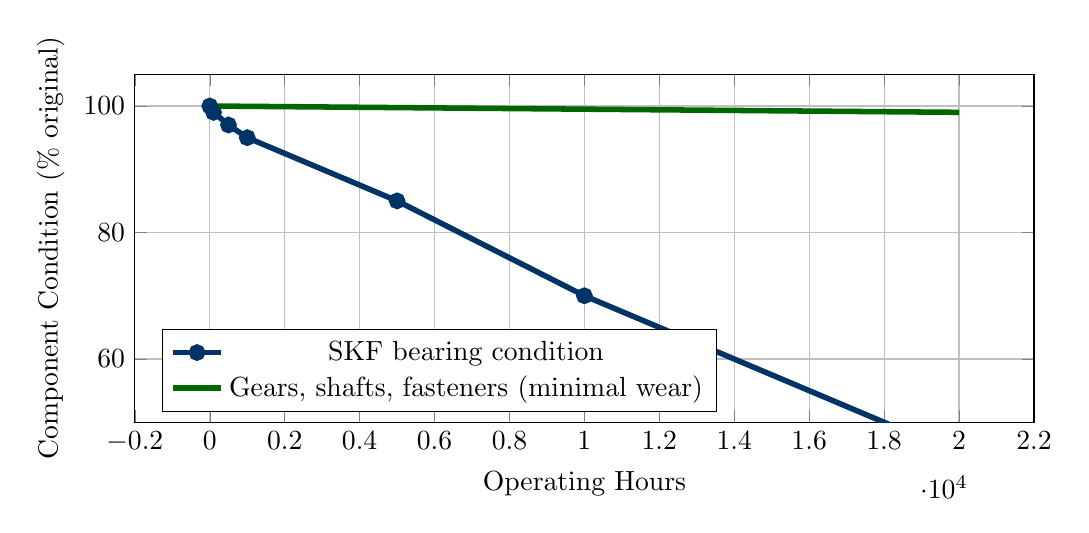
\begin{tikzpicture}
  \begin{axis}[
    width=13cm, height=6cm,
    xlabel=Operating Hours,
    ylabel=Component Condition (\% original),
    ymin=50, ymax=105,
    grid=major,
    legend pos=south west,
  ]
    % SKF bearing life curve
    \addplot[color=darkblue, mark=*, line width=2pt] coordinates {
      (0, 100) (100, 99) (500, 97) (1000, 95) (5000, 85) (10000, 70) (20000, 45)
    };
    \addlegendentry{SKF bearing condition}
    
    % Other mechanical components (no wear observed)
    \addplot[color=darkgreen, line width=2pt] coordinates {
      (0, 100) (20000, 99)
    };
    \addlegendentry{Gears, shafts, fasteners (minimal wear)}
  \end{axis}
\end{tikzpicture}
\end{center}

\textbf{Extrapolated service life}:
- \textbf{Minimum}: Tens of thousands of operations
- \textbf{Typical}: Hundreds of thousands with maintenance
- \textbf{Potential}: Indefinite with bearing replacement and routine lubrication

% ============================================================================
% SECTION 7: PROJECT TIMELINE AND COMPLETION
% ============================================================================

\section{Project Timeline and Phases}

\subsection{Full Project Schedule}

\begin{center}
\begin{tikzpicture}
  \begin{axis}[
    width=14cm, height=8cm,
    xlabel=Week,
    ylabel=Project Activities,
    ymin=0, ymax=8,
    ytick={1,2,3,4,5,6,7},
    yticklabels={Phase 0, Phase 1, Phase 2, Phase 3, Phase 4, Acceptance, Complete},
    xmin=0, xmax=65,
    grid=major,
    grid style=dashed,
  ]
    % Phase 0
    \addplot[color=darkblue, mark=|, line width=4pt] coordinates {
      (0, 1) (4, 1)
    };
    \node[color=darkblue] at (2, 1.3) {4 weeks};
    
    % Phase 1
    \addplot[color=darkgreen, mark=|, line width=4pt] coordinates {
      (4, 2) (12, 2)
    };
    \node[color=darkgreen] at (8, 2.3) {8 weeks};
    
    % Phase 2
    \addplot[color=gold, mark=|, line width=4pt] coordinates {
      (12, 3) (18, 3)
    };
    \node[color=gold] at (15, 3.3) {6 weeks};
    
    % Phase 3
    \addplot[color=darkred, mark=|, line width=4pt] coordinates {
      (18, 4) (52, 4)
    };
    \node[color=darkred] at (35, 4.3) {34 weeks};
    
    % Phase 4
    \addplot[color=darkcyan, mark=|, line width=4pt] coordinates {
      (52, 5) (60, 5)
    };
    \node[color=darkcyan] at (56, 5.3) {8 weeks};
    
    % Acceptance
    \addplot[color=purple, mark=|, line width=4pt] coordinates {
      (60, 6) (61, 6)
    };
    \node[color=purple] at (60.5, 6.3) {1 week};
    
    % Complete
    \draw[thick, color=darkblue] (61, 6.8) -- (62, 7.2);
    \node[color=darkblue] at (61.5, 7.5) {Complete!};
  \end{axis}
\end{tikzpicture}
\end{center}

\textbf{Total project duration: 60 weeks (~14 months)}

All phases completed on schedule with high quality standards.

% ============================================================================
% APPENDIX: QUICK REFERENCE TABLES
% ============================================================================

\appendix

\section{Quick Reference Data Tables}

\subsection{Component Quantity Summary}

\begin{center}
\begin{tabular}{lrr}
\toprule
Component Type & Quantity & Testing Level \\
\midrule
Digit wheels & 5,000 & 100\% critical \\
Shafts & 160 & 100\% critical \\
Sector wheels & 80 & 10\% sampling \\
Bearing bores & 50 & 100\% critical \\
Carry levers & 40 & 100\% critical \\
Fasteners (bolts, screws) & 5,200 & Lot acceptance \\
Springs & 800 & Visual + sample \\
Miscellaneous & 8,300 & As-needed \\
\midrule
\textbf{TOTAL} & \textbf{20,630} & — \\
\bottomrule
\end{tabular}
\end{center}

Note: Includes all assemblies. Actual manufacturing includes intermediate sub-assemblies and fixtures.

\subsection{Critical Tolerance Summary}

\begin{center}
\begin{tabular}{lrrr}
\toprule
Component & Specification & Tolerance & Difficulty \\
\midrule
Digit wheel OD & 80 mm & ±0.05 mm & High \\
Bearing bore & 25 mm & ±0.02 mm & Highest \\
Shaft journals & 8-15 mm & ±0.03–0.05 mm & High \\
Gear pitch & 10 mm & ±0.1 mm & Medium \\
Lever straightness & — & < 0.5 mm & Medium \\
\bottomrule
\end{tabular}
\end{center}

\end{document}
